\documentclass[11pt,reqno]{amsart}
\usepackage[T1]{fontenc}
\usepackage{lmodern,microtype,amsmath,amssymb,mathtools}
\usepackage[a4paper,margin=28mm]{geometry}
\usepackage{booktabs,array,longtable,enumitem,float}
\usepackage{upquote}
\usepackage{tikz}
\usetikzlibrary{arrows.meta,positioning}
\usepackage[hidelinks]{hyperref}
\newtheorem{theorem}{Theorem}[section]
\newtheorem{lemma}[theorem]{Lemma}
\newtheorem{proposition}[theorem]{Proposition}
\newtheorem{corollary}[theorem]{Corollary}
\theoremstyle{definition}
\newtheorem{definition}[theorem]{Definition}
\newtheorem{remark}[theorem]{Remark}
\newcommand{\HG}{\operatorname{HG}_{P}}
\newcommand{\F}{\mathbb{F}}
\newcommand{\ind}{\mathbf{1}}
\newcommand{\calC}{\mathcal{C}}
\newcommand{\calA}{\mathcal{A}}
\newcommand{\calR}{\mathcal{R}}
\newcommand{\calT}{\mathcal{T}}
\newcommand{\sat}{\mathrm{SAT}}
\newcommand{\unsat}{\mathrm{UNSAT}}
\newcommand{\Stirling}[2]{\genfrac{\{}{\}}{0pt}{}{#1}{#2}}
\numberwithin{equation}{section}
\setlist[enumerate]{label=\textup{(\roman*)},leftmargin=*,itemsep=3pt}
\setlength{\emergencystretch}{2em}
\raggedbottom
\title[Proper hat guessing on the five-cycle]{The Proper Hat-Guessing Number of the Five-Cycle:\\A Computer-Assisted Argument}
\author{Shiqi Liu}
\address{Dalian University of Technology}
\date{October 27, 2026 (prepared after local mathematical and computational checks)}
\thanks{Developed with computer and AI assistance; the scope of the local verification and access to its evidence are stated in Sections~\ref{sec:certificates} and~\ref{sec:conclusion}.}
\keywords{Proper hat guessing, cycle, finite classification, satisfiability, proof certificates}
\hypersetup{pdftitle={The Proper Hat-Guessing Number of the Five-Cycle: A Computer-Assisted Argument},pdfauthor={Shiqi Liu},pdfsubject={arXiv submission candidate with versioned computational evidence}}
\begin{document}
\begin{abstract}
We give a computer-assisted proof that the proper hat-guessing number
of the five-cycle is four. The upper bound concerns arbitrary deterministic
local rules, with no symmetry assumption. A counting argument selects a
color guessed on at most 25 strategy-table entries. A classification of
two-vertex covers in a bipartite graph proves the necessary lower bound
17. These restrictions, followed by vertex and color relabeling,
reduce the exclusion to 1413 count representatives and 8613 terminal
Boolean formulas. We separate three obligations: coverage of every
hypothetical strategy, preservation of that strategy by the actual
encoding, and refutation of each terminal formula. The encoding check
exhausts all 65,399 admissible inputs of the 14 counter-component types;
the complete local replay checks 66,403,934 reverse-unit-propagation
additions, including every final empty clause. We give examples of the
reductions, explain the inference rule, and specify how the versioned
code, input and proof records fit together. A local witness attaining 17
shows why the two-occurrence argument alone is insufficient. The
verification uses separately implemented local programs within one
AI-assisted workflow; it is not a proof-assistant formalization.
\end{abstract}
\maketitle
\section{Introduction and the main result}\label{sec:introduction}
In the proper hat-guessing game, the players occupy the vertices of a graph.
Adjacent players must wear different colors. Each player sees the colors
of its neighbors and guesses its own color; all guesses are made
simultaneously, and the players win if at least one guess is correct.
A winning strategy must work for every permitted assignment of hats.
Adriaensen et al.\ introduced this variant and the parameter $\HG(G)$
in~\cite{proper}. Table~1 of the inspected version~4 gives
$4\leq\HG(C_5)\leq5$. We settle this particular alternative by excluding
five colors and recalling an explicit four-color strategy.

Related developments include general upper bounds in terms of order and
maximum degree~\cite{kakatelis}, and coverability methods and exact results
for two-spine book graphs~\cite{zhai}. Here we focus on the five-cycle
and the alternative recorded in Table~1 of the cited version of~\cite{proper}.

\begin{theorem}[Main theorem; computer-assisted]\label{thm:main}
The proper hat-guessing number of the five-cycle is
\[
\HG(C_5)=4.
\]
\end{theorem}

The players may use different rules and distinguish left from right.
Their rules need not be invariant under any permutation of vertices or
colors. Nonadjacent hats may agree, and a permitted configuration need
not use all five colors. Thus the task is to exclude the entire local
strategy space, rather than a symmetric family of candidate rules.

\subsection{The idea of the proof}
There are five strategy tables, each with $5^2=25$ ordered observations.
A guess equal to a neighbor's color is always wrong and can be replaced
without losing any previously correct guess. After this normalization,
each of the 125 table entries contributes to exactly one color's count.
Some color $z$ is therefore guessed on at most 25 entries. Write $S(z)$
for this count; it counts table entries, not successful configurations.

To bound $S(z)$ below, consider configurations in which $z$ occurs twice.
The two players wearing $z$ are nonadjacent. Once the answers of the other
three players are fixed, the pairs of colors they miss form a small
bipartite graph. Its vertex covers describe which entries of the two
remaining tables must guess $z$. Every relevant slice needs at least two
such entries, giving a pairwise bound. Classifying when equality is
possible rules out total counts 15 and 16, and yields $S(z)\geq17$.
This is the combinatorial part of the argument.

The remaining work is finite, but the reduction still needs justification.
Vertex relabeling gives 1413 representatives of the necessary five-player
count vectors with $17\leq S(z)\leq25$. These vectors fix only counts,
not the positions of entries or the remaining answers. Each representative
becomes a Boolean formula describing all still-possible winning strategies.
A direct refutation suffices for 1269 representatives. The other 144 are
refined into 51 color-equality patterns each, giving
\[
1269+144\cdot51=8613
\]
terminal formulas. Each has a checked refutation. The choice of which
parents to refine affects computational cost, not the required coverage.

\begin{figure}[htbp]
\centering
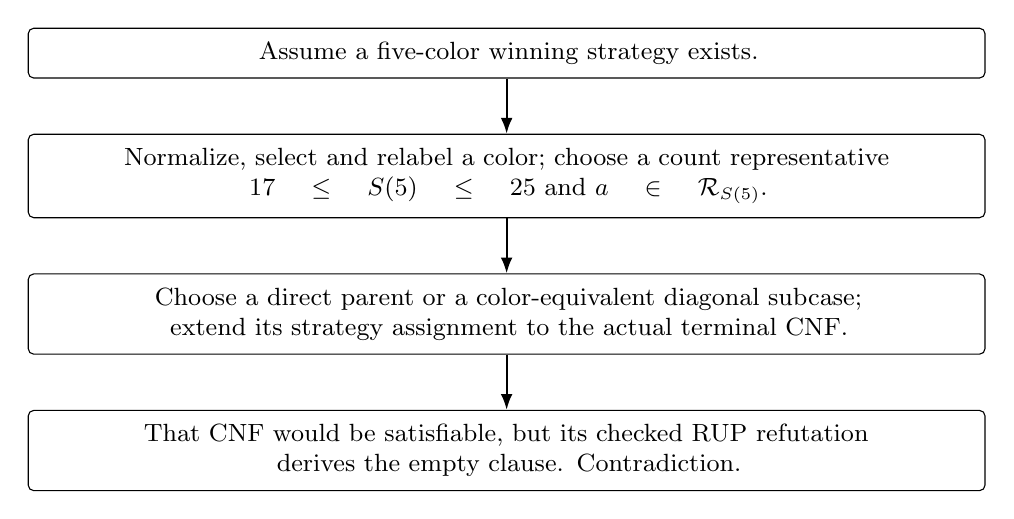
\begin{tikzpicture}[
 stage/.style={draw,rounded corners=2pt,align=center,text width=11.8cm,
                inner sep=5pt,font=\small},
 proofarrow/.style={-{Latex[length=2mm]},thick},node distance=7mm]
\node[stage] (strategy) {Assume a five-color winning strategy exists.};
\node[stage,below=of strategy] (count)
 {Normalize, select and relabel a color; choose a count representative\\
 $17\leq S(5)\leq25$ and $a\in\calR_{S(5)}$.};
\node[stage,below=of count] (formula)
 {Choose a direct parent or a color-equivalent diagonal subcase;\\
 extend its strategy assignment to the actual terminal CNF.};
\node[stage,below=of formula] (conflict)
 {That CNF would be satisfiable, but its checked RUP refutation\\
 derives the empty clause. Contradiction.};
\draw[proofarrow] (strategy)--(count);
\draw[proofarrow] (count)--(formula);
\draw[proofarrow] (formula)--(conflict);
\end{tikzpicture}
\caption{The route from an arbitrary strategy to a contradiction.
The reductions preserve a hypothetical winning strategy; the input audit
checks that the generated clauses preserve its satisfying extension.}
\label{fig:proof-route}
\end{figure}

\subsection{What has to be checked}
The proof has three obligations. Keeping them separate makes clear both
what the computer establishes and why that establishes a result about hats.
\begin{enumerate}
\item \emph{Coverage.} Every hypothetical winning strategy has an
 equivalent representative in a listed branch. The mathematical
 reductions are proved in Sections~\ref{sec:preliminaries}--\ref{sec:classification}.
\item \emph{Preservation.} The representative extends to a satisfying
 assignment of the actual branch input. Section~\ref{sec:encoding}
 proves the logical criterion and explains the exhaustive check of the
 generated auxiliary components.
\item \emph{Exclusion.} Every terminal input has a valid refutation.
 Section~\ref{sec:certificates} proves the soundness of the inference
 rule and states the finite assertion verified on the saved files.
\end{enumerate}
A solver's answer alone cannot establish these three facts. In particular,
a refutation of an incorrectly restricted formula would not exclude all
strategies. Section~\ref{sec:conclusion} assembles the three obligations
into the proof of Theorem~\ref{thm:main}.

The switch from a local argument to the full encoding is necessary for
this approach. Appendix~\ref{app:witness} exhibits a strategy with
$S(5)=17$ that wins on all configurations with two hats of color 5, yet
loses on configurations with zero or one such hat. The full formula
therefore includes all 1020 proper five-colorings, not just the
240 configurations used to obtain the combinatorial lower bound.

\subsection{Evidence and reading guide}
The complete computational audit reported here is the run of
27 October 2026: a new input auditor checked every parent and child
formula, and the frozen \texttt{FreshRup} checker replayed every adopted
terminal proof. Appendix~\ref{app:reproduction} gives the versioned
material list and executable reproduction steps;
Appendix~\ref{app:audit} identifies the run records, file fingerprints,
implementation tests and their precise scope. It distinguishes this
full replay from the smaller checks performed while packaging the evidence.

A reader interested primarily in the mathematics can follow
Sections~\ref{sec:preliminaries}--\ref{sec:encoding}, the RUP soundness
lemma, and the final deduction, treating the explicitly stated finite
verification as the computational premise. A reproducer should then
check the actual input files and complete terminal set, using the
appendix rather than saved success summaries as a substitute for running
the checks.

Separate implementations were used within the same AI-assisted workflow.
They are not independent human peer reviewers, and the checker has not
been formally verified. This paper makes no claim of an exhaustive
novelty search: its comparison with~\cite{proper} refers specifically to
the cited version. The evidence is staged for coordinated public release with this
preprint, as described at the end of Section~\ref{sec:conclusion}.

\section{The model and elementary reductions}\label{sec:preliminaries}
We first specify the full strategy space. The later reductions will select
equivalent candidates from this space, without assuming that the five
players share a rule.
\subsection{Rules and quantifiers}
Let $Q_q=\{1,\ldots,q\}$. The vertices of $C_5$ are $1,\ldots,5$ in cyclic
order; vertex indices are read modulo~5. Set
\[
\calC_q=\{c\in Q_q^5:c_i\ne c_{i+1}\text{ for every }i\}.
\]
In particular, $c_5\ne c_1$ is required. Nonadjacent vertices may have the
same color, and a member of $\calC_q$ need not use all $q$ colors. A
strategy is a tuple $f=(f_1,\ldots,f_5)$, where
\[
f_i:Q_q^2\longrightarrow Q_q.
\]
The first and second arguments are the left and right neighbor colors,
respectively. Winning means
\begin{equation}\label{eq:winning}
\forall c\in\calC_q\quad
\exists i\in\{1,\ldots,5\}\quad
f_i(c_{i-1},c_{i+1})=c_i.
\end{equation}
There is no communication after the colors have been assigned.
Thus the five functions are fixed before the adversary chooses a coloring,
while the player whose guess is correct may depend on that coloring.
We use
\[
\HG(C_5)=\sup\{q\in\mathbb Z_{\geq2}:\text{a winning strategy with $q$ colors exists}\}.
\]
The lower and upper bounds below make this supremum a finite maximum.

\subsection{The four-color strategy and palette restriction}
\begin{lemma}[Restriction of the palette]\label{lem:palette}
If a winning strategy exists with $q$ colors and $2\leq r\leq q$, then a
winning strategy exists with $r$ colors.
\end{lemma}
\begin{proof}
Choose an $r$-element subset $R$ of the palette and restrict attention to
configurations with colors in $R$. On observations in $R^2$, replace any
answer outside $R$ by an arbitrary element of $R$. Such an original answer
could not have been correct on a configuration under consideration, so no
previously correct guess is lost. Relabel $R$ as $Q_r$.
\end{proof}

\begin{proposition}[The four-color lower bound]\label{prop:four}
There is a winning strategy on $C_5$ with four colors.
\end{proposition}
\begin{proof}
Use the path strategy of~\cite[Lemma~4.1]{proper}. Identify the colors with
$\F_2^2$ and write the colors at three consecutive vertices as $a,b,c$.
Their guesses are, respectively,
\[
(b_1+1,b_2),\qquad(c_1+1,a_2+1),\qquad(b_1,b_2+1).
\]
All coordinates and additions in this construction are in $\F_2$.
The end vertices ignore their other neighbor. Suppose both end guesses
fail. Properness excludes $a=(b_1,b_2)$, and failure of the first guess
excludes $a=(b_1+1,b_2)$. These are exactly the two colors with second
coordinate $b_2$, so $a_2=b_2+1$. Similarly, properness and failure of
the third guess exclude $(b_1,b_2)$ and $(b_1,b_2+1)$ for $c$; hence
$c_1=b_1+1$. Substituting these two identities into the middle guess
gives $(b_1+1+1,b_2+1+1)=b$.
The other two players may guess arbitrarily.
\end{proof}

Thus it suffices to exclude five colors. Henceforth $Q=Q_5$.

\subsection{Normalizing and counting table entries}
\begin{center}\small
\begin{tabular}{@{}lp{10.3cm}@{}}
\toprule
Notation&Meaning\\
\midrule
$\calC_q$&All proper colorings of the labeled cycle with palette $Q_q$.\\
$M_i^z$&The $4\times4$ indicator matrix for guessing $z$ when neither
neighbor has color $z$; row = left neighbor, column = right neighbor.\\
$s_i(z),S(z)$&The weight of this matrix and the sum of its weights over all five players.\\
$a_j$&The same five weights in the order $(1,3,5,2,4)$, in which
nonadjacent players are consecutive.\\
\bottomrule
\end{tabular}
\end{center}
The notation is defined formally below; this table fixes the two distinct
orders used in the proof and in the saved data.

\begin{lemma}[Removal of impossible guesses]\label{lem:normalization}
A winning strategy can be replaced by one satisfying
\begin{equation}\label{eq:normalization}
f_i(a,b)\notin\{a,b\}
\qquad(i\in\{1,\ldots,5\},\ a,b\in Q).
\end{equation}
Moreover, for a fixed color $z$, the replacement can preserve every
indicator $\ind[f_i(a,b)=z]$ with $a,b\ne z$.
\end{lemma}
\begin{proof}
If an answer belongs to $\{a,b\}$, it is incorrect in every proper coloring
with that observation. Replacing it by any element of
$Q\setminus\{a,b\}$ loses no correct guess. To preserve the indicated
entries, put $S=Q\setminus\{z\}$. On an observation in $S^2$, replace an
impossible answer by a color in $S\setminus\{a,b\}$; this set has at least
two elements. Neither the old nor the new answer is $z$. On observations
containing $z$, the specified indicators are not defined, so any allowed
replacement may be used. Apply this independently to all affected entries.
\end{proof}

For $z\in Q$, define
\begin{equation}\label{eq:counts}
M_i^z(a,b)=\ind[f_i(a,b)=z]\quad(a,b\in Q\setminus\{z\}),\qquad
s_i(z)=\sum_{a,b\ne z}M_i^z(a,b),\qquad
S(z)=\sum_{i=1}^5s_i(z).
\end{equation}
These counts refer to all five tables, not to the number of correct guesses
on a particular coloring. Each $s_i(z)$ is the weight of a $4\times4$
Boolean matrix and lies between 0 and~16.
For example, $f_i(1,2)=5$ contributes one to $s_i(5)$; it does not
count how many global colorings are won using this answer. This distinction
lets us compare strategies by only five integers while leaving their
table positions free.

\begin{lemma}[The total-count identity]\label{lem:total}
For every strategy, $\sum_zS(z)\leq125$. Under
\eqref{eq:normalization}, equality holds. Consequently, a normalized
winning strategy has a color $z$ with $S(z)\leq25$.
\end{lemma}
\begin{proof}
There are five tables, each with 25 ordered observations. An entry
$f_i(a,b)=g$ contributes to exactly one of the counts in~\eqref{eq:counts}
when $g\notin\{a,b\}$, namely to $s_i(g)$, and contributes to none
otherwise. The final assertion is the pigeonhole principle.
\end{proof}

The fixed-color preservation in Lemma~\ref{lem:normalization} has a
specific quantifier: for each chosen $z$, there is a suitable repair.
It does not assert that one repair preserves all five values $S(z)$
simultaneously. The main argument first makes any normalization and then
chooses a least-used color. The preservation clause is needed when
transferring a lower bound for a specified color back to an unnormalized
strategy, as in Corollary~\ref{cor:balance}.

\subsection{The configuration families}
The number of permitted configurations will also be useful. With $J_q$
the all-ones matrix and $I_q$ the identity matrix, proper cyclic colorings
are the closed walks of length~5 in the color-transition matrix $J_q-I_q$.
Its eigenvalues are $q-1$ once and $-1$ with multiplicity $q-1$, so
\begin{equation}\label{eq:configuration-count}
|\calC_q|=\operatorname{tr}((J_q-I_q)^5)=(q-1)^5-(q-1).
\end{equation}
In particular, $|\calC_5|=1020$ and $|\calC_4|=240$. Vertices are labeled,
so there is no division by~5. The vertices carrying a fixed color form an
independent set of the cycle, of size at most two. The numbers of colorings
with zero, one, and two occurrences of that color are, respectively,
\begin{equation}\label{eq:layers}
240,\qquad 5\cdot4\cdot3^3=540,\qquad5\cdot4\cdot(4\cdot3)=240.
\end{equation}
Indeed, one occurrence leaves a path on four vertices, and two occurrences
must occupy one of the five nonadjacent pairs.
These families will play different roles: the 240 two-occurrence colorings
give the hand-derived lower bound, whereas the Boolean model retains all
$240+540+240=1020$ colorings.


\section{A combinatorial lower bound for a fixed color}\label{sec:local}
Fix $z\in Q$ and put $S=Q\setminus\{z\}$. By
Lemma~\ref{lem:normalization}, we may work with a normalized strategy
without changing the matrices $M_i^z$. Throughout this section it is enough
to require winning only on the configurations in which $z$ occurs twice.
The argument proceeds from one fixed nonadjacent pair of $z$-vertices
to all five such pairs. We first obtain a pairwise inequality, then
analyze equality, and finally show that total weights 15 and 16 would
force incompatible equality cases.

\subsection{A missed-pair graph}
Fix two nonadjacent vertices $i,i+2$ and write a configuration in cyclic
order starting at $i$ as
\begin{equation}\label{eq:two-z}
(z,u,z,v,w),\qquad u,v,w\in S,\quad v\ne w.
\end{equation}
Set
\[
t=f_{i+1}(z,z),\qquad
\alpha(w)=f_{i+3}(z,w),\qquad
\beta(v)=f_{i+4}(v,z).
\]
Normalization gives $t\in S$, $\alpha(w)\in S\setminus\{w\}$, and
$\beta(v)\in S\setminus\{v\}$. Define
\begin{equation}\label{eq:missed}
E=\{(v,w)\in S^2:v\ne w,\ \alpha(w)\ne v,\ \beta(v)\ne w\}.
\end{equation}
The variables $u,v,w$ describe actual hat colors, whereas $t,\alpha,\beta$
are answers supplied by the strategy. The five observations give:
\begin{center}\small
\begin{tabular}{@{}cccl@{}}
\toprule
Player&Hat&Observation&Condition for a correct guess\\
\midrule
$i$&$z$&$(w,u)$&$M_i^z(w,u)=1$\\
$i+1$&$u$&$(z,z)$&$u=t$\\
$i+2$&$z$&$(u,v)$&$M_{i+2}^z(u,v)=1$\\
$i+3$&$v$&$(z,w)$&$\alpha(w)=v$\\
$i+4$&$w$&$(v,z)$&$\beta(v)=w$\\
\bottomrule
\end{tabular}
\end{center}
View $E$ as a bipartite graph whose row vertices are labeled by $v$ and whose
column vertices are labeled by $w$. Among the 12 ordered unequal pairs,
$\alpha$ guesses exactly four and $\beta$ guesses exactly four. Their sets
may intersect, so
\begin{equation}\label{eq:missed-size}
|E|\geq4.
\end{equation}
Every vertex of this graph has degree at most~3; in particular, one vertex
cannot cover all its edges. Notice that $E$ does not depend on~$u$.
Even when a row and a column have the same color label, they are distinct
vertices of this bipartite graph. A vertex cover is a set of row and
column vertices meeting every edge; it is not a set of colors.

For $u\ne t$, the middle player in~\eqref{eq:two-z} is wrong. For
$(v,w)\in E$, both end players are wrong as well. Thus one of the two
players wearing $z$ must be correct, which is equivalent to
\begin{equation}\label{eq:slice-cover}
M_i^z(w,u)=1\quad\text{or}\quad M_{i+2}^z(u,v)=1.
\end{equation}
For a fixed $u$, define the graph vertices selected by these two tables as
\[
R_u=\{v\in S:M_{i+2}^z(u,v)=1\},\qquad
C_u=\{w\in S:M_i^z(w,u)=1\}.
\]
Condition~\eqref{eq:slice-cover} says exactly that
$E\subseteq(R_u\times S)\cup(S\times C_u)$: the rows $R_u$ and columns
$C_u$ form a vertex cover of~$E$.
The graph's column label $w$ is the \emph{row} index of $M_i^z$, and its
row label $v$ is the \emph{column} index of $M_{i+2}^z$; both follow from
the actual observations in the table above. The cover size $|R_u|+|C_u|$
is therefore the number of ones in column $u$ of $M_i^z$ plus the number
in row $u$ of $M_{i+2}^z$. Different values of $u$ use disjoint matrix
entries, so the three cover bounds can be added without double counting.

For a concrete picture, take $S=\{1,2,3,4\}$ and give both $\alpha$ and
$\beta$ the value list $(2,3,4,2)$ on inputs $1,2,3,4$. The missed pairs
are the four dots below; dashes mark the forbidden equal-color pairs.
\[
\begin{array}{c|cccc}
v\backslash w&1&2&3&4\\\hline
1&-& &\bullet&\bullet\\
2& &-& & \\
3&\bullet& &-& \\
4&\bullet& & &-
\end{array}
\qquad
E=\{(1,3),(1,4),(3,1),(4,1)\}.
\]
Selecting row~1 and column~1 covers every dot. In a slice $u\ne t$ this
choice means $M_{i+2}^z(u,1)=M_i^z(1,u)=1$. The two selected vertices
have the same color label but control two different players' guesses.
This example illustrates the correspondence; the following lemmas handle
every allowed pair of functions $\alpha,\beta$.

\begin{lemma}[Pair inequality]\label{lem:pair}
For every $i$,
\[
s_i(z)+s_{i+2}(z)\geq6.
\]
Consequently, $S(z)\geq15$.
\end{lemma}
\begin{proof}
For each of the three choices $u\in S\setminus\{t\}$, a vertex cover as
in~\eqref{eq:slice-cover} has at least two vertices by
\eqref{eq:missed-size}. Hence
\[
\sum_{w\in S}M_i^z(w,u)+\sum_{v\in S}M_{i+2}^z(u,v)\geq2.
\]
Sum over these three values of $u$ and include the nonnegative contribution
at $u=t$. This gives the pair inequality. Summing it over the five values
of $i$ counts every $s_i(z)$ twice and gives $2S(z)\geq30$.
\end{proof}

\subsection{All vertex covers of size two}
The bound 15 used only the fact that each of three slices needs at least
two selected entries. To improve it, we must understand equality: a matrix
participates in two different pair inequalities, so the equality shapes
forced by those pairs must be compatible. We first classify the covers
that a tight slice can use.

\begin{lemma}[Two-vertex covers]\label{lem:covers}
For a graph $E$ defined by~\eqref{eq:missed}, the following hold.
\begin{enumerate}
\item A cover consisting of a row $a$ and a column $b$ is possible only
when $a=b$. If it exists, it is the unique cover of size two, and $E$ is
the disjoint union of two copies of $K_{1,2}$ centered at that row and column.
\item There is at most one cover consisting of two rows and at most one
consisting of two columns.
\item If both pure covers exist, $E$ consists of all four edges of the
resulting $2\times2$ rectangle, and its row-label and column-label sets are
disjoint.
\end{enumerate}
\end{lemma}
\begin{proof}
\emph{Mixed covers with different labels.}
Suppose that row $a$ and column $b$, with $a\ne b$, cover $E$. The submatrix
on $S\setminus\{a\}$ and $S\setminus\{b\}$ contains nine pairs. Exactly two
are diagonal pairs, since $|S\setminus\{a,b\}|=2$, leaving seven permitted
unequal pairs. None may belong to $E$. However, $\alpha$ can cover at most
one pair in each of the remaining three columns, and $\beta$ can cover at
most one in each of the three rows. Together they cover at most six, a
contradiction.

\emph{Mixed covers with the same label.}
Now suppose that row $a$ and column $a$ cover $E$, and let
$T=S\setminus\{a\}$. The six unequal pairs in $T^2$ must all be covered
by $\alpha$ or $\beta$. Each function covers at most three such pairs.
Thus both cover exactly three, their covered sets are disjoint, and
$\alpha(T),\beta(T)\subseteq T$. In column $a$, the three legal rows lie
in $T$. The function $\beta$ guesses $a$ at none of these rows, while
$\alpha(a)\in T$ covers exactly one of the three pairs. Exactly two edges
of $E$ remain in column $a$. In row $a$, the function $\alpha$ never
answers $a$ in columns of $T$, and $\beta(a)\in T$ covers exactly one
of its three legal cells. Exactly two edges therefore remain in row $a$
as well. There are no other edges. The two stars have disjoint
vertex sets. A cover of a two-edge star that uses only one vertex must use
its center, so their two centers are the unique cover of size two.

\emph{Pure covers.}
If two distinct pairs of rows each cover $E$, every row incident with an
edge belongs to the intersection of the two pairs, which has size at most
one. This would give at most three edges, contradicting~\eqref{eq:missed-size}.
The same reasoning applies to columns. Finally, if a pair of rows and a
pair of columns both cover $E$, all edges lie in their $2\times2$ rectangle.
There are at least four edges, so every cell is an edge. A shared color
label between the two pairs would put a forbidden diagonal cell in this
rectangle. The label sets must therefore be disjoint.
\end{proof}

\subsection{Tight pairs and consecutive equalities}
The support of a Boolean matrix is called an $r\times s$ full rectangle
if it is the product of an $r$-element row set and an $s$-element column
set. In the following statement a rectangle with a zero dimension is empty.
Thus its weight is $rs$; for a nonempty rectangle, $r$ and $s$ are the
numbers of nonzero rows and columns in the fixed left/right convention.

\begin{lemma}[Structure of a tight pair]\label{lem:tight}
If $s_i(z)+s_{i+2}(z)=6$, then either
\begin{enumerate}
\item the supports of $M_i^z,M_{i+2}^z$ are full rectangles of sizes
$1\times3$ and $3\times1$, respectively; or
\item for some $k\in\{0,1,2,3\}$ they are full rectangles of sizes
$2\times k$ and $(3-k)\times2$, respectively.
\end{enumerate}
In particular,
\begin{equation}\label{eq:tight-counts}
(s_i(z),s_{i+2}(z))\in\{(0,6),(2,4),(3,3),(4,2),(6,0)\}.
\end{equation}
\end{lemma}
\begin{proof}
In the proof of Lemma~\ref{lem:pair}, the three slices $u\ne t$ must each
contribute exactly two entries, and the slice $u=t$ must contribute zero.
Each selected pair is therefore a cover of $E$ of size two.
There are no additional nonzero entries outside these covers: their
three contributions already account for the entire weight six.

If a mixed cover exists, Lemma~\ref{lem:covers} makes it unique: row $a$
and column $a$ for some $a\in S$. Thus $M_i^z(a,u)=1$ for all $u\ne t$,
and these are its only nonzero entries. Likewise, the only nonzero entries
of $M_{i+2}^z$ are $M_{i+2}^z(u,a)=1$ for $u\ne t$. This gives (i).

If there is no mixed cover, each slice chooses either the unique pure
column cover, when available, or the unique pure row cover. Let $U$ be the
set of slices using the column cover and put $k=|U|$. The nonzero entries
of $M_i^z$ have row labels equal to the two selected column labels of $E$
and column labels in $U$. The nonzero entries of $M_{i+2}^z$ have row
labels in $(S\setminus\{t\})\setminus U$ and column labels equal to the
two selected row labels of $E$. This proves (ii), including the cases in
which only one pure cover is available. When $k=0$ or $k=3$, the
unused cover need not exist; the corresponding matrix is empty, and
its zero-dimensional rectangle denotes just the empty support.
Counting entries gives
\eqref{eq:tight-counts}.
\end{proof}

\begin{corollary}[A restriction at two tight pairs]\label{cor:two-tight}
If $s_{i-2}(z)+s_i(z)=s_i(z)+s_{i+2}(z)=6$, then
$s_i(z)\in\{0,4\}$.
\end{corollary}
\begin{proof}
By~\eqref{eq:tight-counts}, the candidates are $0,2,3,4,6$. In the pair
$(i-2,i)$ the matrix $M_i^z$ is the right-hand matrix of
Lemma~\ref{lem:tight}, whereas in the pair $(i,i+2)$ it is the left-hand
matrix. For weights 2, 3, and 6, its required dimensions in these two roles
are, respectively,
\[
\begin{array}{c|ccc}
\text{weight}&2&3&6\\\hline
\text{right-hand role}&1\times2&3\times1&3\times2\\
\text{left-hand role}&2\times1&1\times3&2\times3
\end{array}
\]
A fixed nonempty matrix cannot have two different numbers of nonzero rows
or columns. These three weights are excluded, leaving only 0 and~4.
\end{proof}

\begin{proposition}[The lower bound 17]\label{prop:seventeen}
Every five-color winning strategy satisfies $S(z)\geq17$ for each $z\in Q$.
\end{proposition}
\begin{proof}
Put $a_j=s_{1+2j}(z)$ for $j\in\mathbb Z/5\mathbb Z$. Thus the player
order is $(1,3,5,2,4)$, and $a_j+a_{j+1}\geq6$. Lemma~\ref{lem:pair}
already gives $\sum_j a_j\geq15$.

\emph{Total 15.}
If $\sum_j a_j=15$, all five pair inequalities are equalities. The equations
$a_{j+1}=6-a_j$ around an odd cycle force every $a_j=3$, contradicting
Corollary~\ref{cor:two-tight}.

\emph{Total 16.}
If $\sum_j a_j=16$, put $e_j=a_j+a_{j+1}-6$. Summing gives
$\sum_j e_j=2\sum_j a_j-30=2$. Such a nonnegative integer vector has
either one entry 2 or two entries 1. In the latter case their positions
on a five-cycle are adjacent or nonadjacent; rotations and reflections
identify all choices of each kind. These are exactly three cases.
Alternating the five pair equations gives
\[
2a_0=(6+e_0)-(6+e_1)+(6+e_2)-(6+e_3)+(6+e_4),
\quad a_{j+1}=6+e_j-a_j.
\]
The following table keeps the same index choices in both columns:
\begin{center}\small
\begin{tabular}{@{}ccc@{}}
\toprule
$(e_0,e_1,e_2,e_3,e_4)$&$(a_0,a_1,a_2,a_3,a_4)$&Forbidden center\\
\midrule
$(2,0,0,0,0)$&$(4,4,2,4,2)$&$a_2=2$\\
$(1,1,0,0,0)$&$(3,4,3,3,3)$&$a_3=3$\\
$(1,0,1,0,0)$&$(4,3,3,4,2)$&$a_4=2$\\
\bottomrule
\end{tabular}
\end{center}
Each indicated center has both incident pair sums equal to six, but its
value is neither 0 nor 4. Corollary~\ref{cor:two-tight} excludes all
three cases. Thus 16 is impossible as well.

\emph{Return to the original strategy.}
For each specified $z$, the count-preserving normalization of
Lemma~\ref{lem:normalization} leaves every $M_i^z$ unchanged. The lower
bound just proved therefore holds for that same $S(z)$ in the original
strategy. Different colors may use different normalizations.
\end{proof}

\subsection{What the local bound does and does not prove}
The argument above uses only 240 of the 1020 proper colorings. The value
17 is sharp for that restricted requirement: Appendix~\ref{app:witness}
gives explicit tables winning on all two-occurrence colorings and having
$S(5)=17$. That same completion loses on other colorings. Thus a larger
lower bound for a full winning strategy must use additional information,
including compatibility with the zero- and one-occurrence families.
The next sections do this by keeping every proper coloring in the base
formula while fixing only the five counts. They do not freeze the
positions or the non-special answers of the local witness.


\section{Complete finite classification}\label{sec:classification}
We now retain only the necessary information proved in the preceding
section. The resulting classes are deliberately larger than the set of
winning strategies. Excluding all of them will therefore exclude every
winning strategy, even though some listed vectors may be unrealizable
for reasons not used in the classification.
\subsection{Count representatives}
The main argument will use a color with $17\leq S(z)\leq25$.
We write $a_j=s_{1+2j}(z)$, so consecutive coordinates correspond to
nonadjacent players. In this order the necessary conditions have a uniform
cyclic form.
For an integer $n$, let $\calA_n$ be the set of integer vectors
$a=(a_0,\ldots,a_4)$ satisfying
\begin{align}
0\leq a_j\leq16,\qquad&\sum_{j=0}^4a_j=n,\label{eq:A1}\\
a_j+a_{j+1}&\geq6,\label{eq:A2}\\
a_j+a_{j+1}=6\quad&\Longrightarrow\quad
(a_j,a_{j+1})\in\{(0,6),(2,4),(3,3),(4,2),(6,0)\},\label{eq:A3}\\
a_{j-1}+a_j=a_j+a_{j+1}=6\quad&\Longrightarrow\quad
a_j\in\{0,4\}.\label{eq:A4}
\end{align}
All indices in these conditions are modulo~5. The range and total are
the definitions of the counts; \eqref{eq:A2} is Lemma~\ref{lem:pair},
\eqref{eq:A3} is Lemma~\ref{lem:tight}, and \eqref{eq:A4} is
Corollary~\ref{cor:two-tight}. No claim of sufficiency is needed.

Let $D_5$ act on these vectors by cyclic shifts and reversal. Choose the
representative that minimizes the ordered pair
\begin{equation}\label{eq:canonical}
\bigl(a_0+a_1,(a_0,a_1,a_2,a_3,a_4)\bigr)
\end{equation}
lexicographically, and denote the set of representatives by $\calR_n$.
The first component of~\eqref{eq:canonical} is an ordering convention
that places a least pair sum first; it is not an additional restriction.
After one representative has been selected from each orbit, the saved
list is sorted lexicographically by the five-tuple itself. This
serialization order is distinct from the key used to select a
representative; set equality and absence of duplicates determine coverage.

\begin{lemma}[Validity of the graph reduction]\label{lem:dihedral}
Every winning strategy with $S(z)=n$ has an equivalent strategy whose
count vector in the order $(1,3,5,2,4)$ belongs to $\calR_n$.
\end{lemma}
\begin{proof}
The count vector belongs to $\calA_n$ by the results of
Section~\ref{sec:local}. A rotation of the vertices transports the five
functions in their cyclic order. A reflection transports the functions
and interchanges their left and right arguments. In either case proper
colorings are carried bijectively to proper colorings, and correct guesses
are preserved. On the matrices, reflection includes transposition, which
preserves their weights. The action on the order $(1,3,5,2,4)$ is again all
cyclic shifts and reversals: multiplication by 2 is invertible modulo~5.
Thus an automorphism sends the count vector to its representative without
requiring any invariance of the strategy itself.
\end{proof}

Explicitly, use vertex labels in $\mathbb Z/5\mathbb Z$ temporarily. A rotation
$h(i)=i+d$ transports rules by $g_{h(i)}(u,v)=f_i(u,v)$; a reflection
$h(i)=d-i$ transports them by $g_{h(i)}(u,v)=f_i(v,u)$. For
$c'_{h(i)}=c_i$, both formulas give
$g_{h(i)}(c'_{h(i)-1},c'_{h(i)+1})=f_i(c_{i-1},c_{i+1})$.
Thus each individual correct guess is preserved. In the count order
$i=1+2j$, the induced actions are $j\mapsto j+k$ and $j\mapsto k-j$.

\subsection{Enumerating the representatives}
There are two elementary ways to produce the entire list. One enumerates
$(a_0,a_1,a_2,a_3)\in\{0,\ldots,16\}^4$, sets
$a_4=n-a_0-a_1-a_2-a_3$, and checks~\eqref{eq:A1}--\eqref{eq:A4}. A
different enumeration uses slack variables
\begin{equation}\label{eq:slack}
e_j=a_j+a_{j+1}-6,\qquad e_j\geq0,\qquad\sum_je_j=2n-30.
\end{equation}
Write $b_j=6+e_j$. The equations $a_j+a_{j+1}=b_j$ have the unique solution
\begin{equation}\label{eq:inverse}
2a_0=b_0-b_1+b_2-b_3+b_4,\qquad
a_{j+1}=b_j-a_j\quad(0\leq j<4).
\end{equation}
Enumerating all compositions of $2n-30$ into five nonnegative parts,
applying~\eqref{eq:inverse}, and testing~\eqref{eq:A1}--\eqref{eq:A4}
therefore gives exactly the same set $\calA_n$. An odd numerator in
\eqref{eq:inverse} is rejected. The last cyclic equation follows from the
formula for $a_0$; the total sum is also checked explicitly in the audit.
This establishes completeness of both enumeration schemes.

For example, the list at weight 17 consists of
\[
\calR_{17}=\{(2,4,3,3,5),\ (2,4,4,2,5),\ (3,3,4,3,4)\}.
\]
The middle vector specifies player counts $(2,2,4,5,4)$ in the ordinary
order $(1,2,3,4,5)$, but fixes none of the locations of the counted entries.
It is also the count vector of the local witness in Appendix~\ref{app:witness}.
In particular, a count branch contains many possible strategies; the
displayed witness is only one table assignment with those counts.

\subsection{Color relabeling and 51 diagonal patterns}
A permutation $\sigma$ of $Q$ acts on strategies by
\begin{equation}\label{eq:color-action}
f_i^\sigma(a,b)=
\sigma\bigl(f_i(\sigma^{-1}(a),\sigma^{-1}(b))\bigr).
\end{equation}
It preserves properness and correctness of each guess. After making the
chosen color equal to 5, permutations of the remaining four colors preserve
every $s_i(5)$. In particular, since $f_1(5,5)\ne5$, we may impose
\begin{equation}\label{eq:one-unit}
f_1(5,5)=1.
\end{equation}
No second normalization involving a different observation is imposed in
the count-branch inputs.
The word ``diagonal'' refers to the observation $(5,5)$ in a player's
table. The two observed vertices are not adjacent to one another, so this
observation is permitted in a proper coloring.

\begin{lemma}[Diagonal-pattern reduction]\label{lem:patterns}
Let $t_i=f_i(5,5)\in\{1,2,3,4\}$. Up to a common permutation of these
four colors, $(t_1,\ldots,t_5)$ is one of the 51 words satisfying
\begin{equation}\label{eq:rgs}
t_1=1,\qquad
1\leq t_j\leq\min\{4,1+\max_{\ell<j}t_\ell\}\quad(2\leq j\leq5).
\end{equation}
This normalization preserves the count representative already chosen.
\end{lemma}
\begin{proof}
Assign the label 1 to the first color encountered in the word, label 2 to
the next previously unseen color, and so forth. Extend this assignment
arbitrarily to a permutation of all four colors. The resulting word
satisfies~\eqref{eq:rgs}. Conversely, its equality classes determine it
uniquely. These words correspond to partitions of five labeled positions
into at most four nonempty blocks. The recurrence
$\Stirling{n}{k}=k\Stirling{n-1}{k}+\Stirling{n-1}{k-1}$ gives
\[
\Stirling{5}{1}+\Stirling{5}{2}+\Stirling{5}{3}+\Stirling{5}{4}
=1+15+25+10=51.
\]
The permutation fixes color 5, so it only permutes the 16 observations
inside each $M_i^5$ and preserves its weight. If~\eqref{eq:one-unit}
already holds, the first-occurrence relabeling fixes its answer~1.
\end{proof}

For example, the word $(1,4,1,2,4)$ has equality blocks
$\{1,3\}$, $\{2,5\}$, and $\{4\}$. Relabeling its first, second, and
third distinct answers as $1,2,3$ gives $(1,2,1,3,2)$.
This is one common permutation applied to every strategy table, not five
independent changes of the players' answers. It preserves color~5 and
the already imposed answer $f_1(5,5)=1$.

\subsection{Why every candidate reaches a listed branch}
\begin{proposition}[Coverage of all five-color candidates]\label{prop:coverage}
If a five-color winning strategy exists, there are
$n\in\{17,\ldots,25\}$ and $a\in\calR_n$ such that an equivalent
normalized winning strategy has count vector $a$ and satisfies
\eqref{eq:one-unit}. For any such count branch selected for refinement,
at least one of the 51 constraints~\eqref{eq:rgs} still contains an
equivalent winning strategy.
\end{proposition}
\begin{proof}
Normalize by Lemma~\ref{lem:normalization}, choose a color with total at
most 25 by Lemma~\ref{lem:total}, and relabel it as~5.
Proposition~\ref{prop:seventeen} supplies the lower bound 17. Apply
Lemma~\ref{lem:dihedral}, then a color permutation fixing 5 to obtain
\eqref{eq:one-unit}. If the branch is refined, apply
Lemma~\ref{lem:patterns}. Each step preserves winning and all count
conditions needed by the next step.
\end{proof}

The order of the two reductions matters. First a vertex automorphism
selects the count representative; next a permutation of the four
non-special colors selects the diagonal representative without changing
any count. The latter operation therefore cannot undo the former. There
is no requirement that the diagonal tuple also be minimal under vertex
automorphisms.

Accordingly, the 51 subcases cover strategy \emph{orbits} under the proved
color action. They need not contain every labeled diagonal word as a
literal assignment. This is a change to an equivalent candidate, not a
symmetry requirement on the five unknown functions. In the next section,
the transformed candidate will be assigned its own auxiliary variables.


\section{Boolean encoding and preservation of candidates}\label{sec:encoding}
A formula in conjunctive normal form (CNF) is an AND of clauses, each
clause being an OR of literals. The encoding is built in three layers:
choose one answer at each observation, require a correct answer on every
proper coloring, then impose the selected branch counts and diagonal
answers. The first two layers describe the game exactly. The last uses
auxiliary variables, for which we need a preservation statement: a
hypothetical winning strategy in the branch must extend to a satisfying
assignment of the actual saved CNF.
\subsection{The base formula}
For a vertex $i\in\{1,\ldots,5\}$ and colors $a,b,g\in Q$ with
$g\notin\{a,b\}$,
introduce a Boolean variable
\[
x_{i,a,b,g}\quad\text{meaning}\quad f_i(a,b)=g.
\]
At each observation $(i,a,b)$ impose the clauses
\begin{align}
&\bigvee_{g\notin\{a,b\}}x_{i,a,b,g},\label{eq:at-least-one}\\
&\neg x_{i,a,b,g}\lor\neg x_{i,a,b,h}
\quad(g<h,\ g,h\notin\{a,b\}).\label{eq:at-most-one}
\end{align}
For every $c\in\calC_5$, add the coverage clause
\begin{equation}\label{eq:coverage-clause}
\bigvee_{i=1}^5x_{i,c_{i-1},c_{i+1},c_i}.
\end{equation}
All its variables exist because $c$ is proper. Let $\Phi$ be the
conjunction of these clauses.

For example, the proper coloring $(5,1,5,2,3)$ contributes the clause
\[
x_{1,3,1,5}\lor x_{2,5,5,1}\lor x_{3,1,2,5}
\lor x_{4,5,3,2}\lor x_{5,2,5,3}.
\]
Its five alternatives say exactly that player 1, 2, 3, 4 or 5 guesses
correctly on this coloring. The diagonal observation $(5,5)$ at player 2
is legitimate because only adjacent vertices must have different colors.

\begin{lemma}[Exactness of the base encoding]\label{lem:base}
The satisfying assignments of $\Phi$ are in bijection with normalized
five-color winning strategies.
\end{lemma}
\begin{proof}
Clauses~\eqref{eq:at-least-one} and~\eqref{eq:at-most-one} select exactly
one allowed answer at each observation, determining a unique normalized
strategy. Clause~\eqref{eq:coverage-clause} holds precisely when at least
one player guesses correctly on its indexed configuration. There is one
such clause for every member of $\calC_5$, so their conjunction is exactly
\eqref{eq:winning}. Conversely, a normalized winning strategy sets its
selected answer variables to true and satisfies all these clauses.
\end{proof}

For each player there are five equal-color observations with four allowed
answers and twenty unequal-color observations with three allowed answers.
The formula therefore has
\[
5(5\cdot4+20\cdot3)=400
\]
variables. The number of selection clauses is
\[
5\left[5\left(1+\binom42\right)+20\left(1+\binom32\right)\right]=575.
\]
Together with the 1020 coverage clauses, this gives 1595 clauses. In
particular, equal-color neighbor observations and colorings using fewer
than five colors have not been omitted.

\subsection{The count-branch formula}
Fix $a\in\calR_n$, and write $r_i=a_j$ when $i=1+2j$ modulo~5.
The intended additional constraints are
\begin{equation}\label{eq:cardinality}
\sum_{u,v\in\{1,2,3,4\}}x_{i,u,v,5}=r_i
\quad(1\leq i\leq5),\qquad x_{1,5,5,1}=1.
\end{equation}
They fix only five counts and one permissible normalization. In
particular, no positions of the $r_i$ selected entries and no other answer
values are fixed.

The recorded implementation uses PySAT sequential-counter components
for the five equalities~\cite{pysat}. Each component has exactly the
16 listed input variables and its own auxiliary variables. Denote the
actual generated component by $K_{i,r_i}(X_i,Y_i)$, where
$X_i=(x_{i,u,v,5})_{u,v\in\{1,2,3,4\}}$ and the $Y_i$ are disjoint.
The actual parent formula is
\begin{equation}\label{eq:parent}
F_a=\Phi\land x_{1,5,5,1}\land\bigwedge_{i=1}^5K_{i,r_i}(X_i,Y_i).
\end{equation}
For a refined parent, the formula at pattern $t\in\calT$, where $\calT$
is defined by~\eqref{eq:rgs}, is exactly
\begin{equation}\label{eq:child}
F_{a,t}=F_a\land\bigwedge_{i=1}^5x_{i,5,5,t_i}.
\end{equation}
The first of these five units duplicates the normalization in $F_a$ and
is harmless.

For the weight-17 example $a=(2,4,4,2,5)$, the counter targets are
$(r_1,r_2,r_3,r_4,r_5)=(2,2,4,5,4)$. In a possible refinement such as
$t=(1,2,1,3,2)$, the answers at $(5,5)$ are fixed to those five values,
while every other answer remains subject only to the base formula and
counts. Fixing a count is therefore different from fixing a table.

\subsection{Why auxiliary encodings do not discard a true strategy}
The required direction for an impossibility proof is
\begin{equation}\label{eq:extension}
\left(\sum X_i=r_i\right)
\ \Longrightarrow\ \exists Y_i\ K_{i,r_i}(X_i,Y_i).
\end{equation}
Accidentally removing an intended input could invalidate an exclusion
proof. Admitting extra inputs makes exclusion harder, but a refutation
would still exclude every intended input. Thus the reverse implication
is not needed. The audit checks~\eqref{eq:extension} on every intended
input of each actual component type, rather than relying only on a
library's claim of exactness. We do not assert a bijection between
strategies and auxiliary assignments; Lemma~\ref{lem:base} concerns only
the base formula.

For this check, the 16 input variables are renamed $1,\ldots,16$, and the
component's auxiliary variables are renamed consecutively from~17. A
component type is identified by its count and its complete normalized
clause list, not just by the count. After a particular input assignment
has been substituted, each remaining clause has at most one positive
auxiliary literal. This Horn property is checked from the actual clauses.

Under substitution, a clause with a true input literal is discarded;
false input literals are removed from the remaining clauses. A remaining
clause $\neg y_1\lor\cdots\lor\neg y_k\lor y$ is the rule
$y_1\land\cdots\land y_k\Rightarrow y$. With no positive literal its
head is $\bot$; with no negative literals it is a fact. This also covers
unit clauses and empty residual clauses.

\begin{lemma}[Auxiliary extension check]\label{lem:horn}
For a fixed input assignment, suppose the residual auxiliary formula is
Horn. Start with no auxiliary variable true. Repeatedly apply every rule
\[
y_{j_1}\land\cdots\land y_{j_k}\ \Longrightarrow\ y_\ell
\]
whose premises are true. Treat a clause with no positive literal as the
same rule with conclusion $\bot$. If closure is reached without deriving
$\bot$, setting exactly the derived variables true satisfies the residual
formula.
\end{lemma}
\begin{proof}
There are finitely many variables, and every successful application adds
a previously false variable, so the process terminates. At closure, a
rule with all premises true has its head true. A rule with head $\bot$
cannot have all premises true. Hence every residual Horn clause is
satisfied. Clauses already satisfied by the fixed input remain satisfied,
so this assignment also satisfies the original component.
\end{proof}

The implementation additionally evaluates every original component clause
on the constructed assignment. For count $r$, it enumerates every
$r$-element subset of the 16 input positions, with no sampling. It checks
the variable ranges and clause intervals to ensure that no component uses
another component's auxiliary variables or unrelated strategy variables.
Consequently, the five separate auxiliary assignments can be combined.

\begin{proposition}[Preservation by a branch input]\label{prop:input}
Suppose the base clauses, variable lists, extra units, and all properties
\eqref{eq:extension} have been checked for a branch. Every normalized
winning strategy in that branch extends to a satisfying assignment of
its actual formula~\eqref{eq:parent} or~\eqref{eq:child}.
\end{proposition}
\begin{proof}
Lemma~\ref{lem:base} supplies a satisfying assignment of $\Phi$.
The strategy satisfies the branch counts and the normalization, so
\eqref{eq:extension} supplies an auxiliary assignment for each component.
The auxiliary sets are disjoint, so their union satisfies all five
components simultaneously. In a refined branch the strategy also
satisfies its five diagonal units.
\end{proof}

This extension is chosen \emph{after} all vertex and color relabelings.
In particular, applying Lemma~\ref{lem:patterns} changes the base
assignment, and we then choose new auxiliary values for that assignment.
No assertion that a sequential-counter formula is syntactically
equivariant under color permutations is needed.

The input audit reconstructs~\eqref{eq:at-least-one}--\eqref{eq:coverage-clause}
directly from the game, compares the base clause multiset, checks all five
component boundaries, and confirms that the only other parent clause is
$x_{1,5,5,1}$. Every child is compared clause by clause with its parent
plus the five specified units. These checks address the mathematical input
to the solver, separately from any subsequent refutation.


\section{Refutations and the finite verification}\label{sec:certificates}
A SAT solver is used to find a refutation; a separate checker establishes
that the saved refutation is valid for the saved input. The distinction is
useful because the search may be complicated, whereas the inference rule
checked at each proof step is elementary. The complete computation used
here has three outputs: a covering list of branches, validated Boolean
inputs for those branches, and a checked refutation for each terminal input.

\subsection{What one proof step means}
Given clauses $D$, \emph{unit propagation} repeatedly sets the sole
unassigned literal of a clause to true when its other literals are false.
An empty clause or conflicting forced assignments gives a contradiction.
For example, from $(p\lor q)$ and $\neg p$, the temporary assumption
$\neg q$ forces $p$ and a conflict. Thus $D$ entails the unit clause $q$.

\begin{definition}
A clause $C=\ell_1\lor\cdots\lor\ell_k$ has the
\emph{reverse-unit-propagation} (RUP) property with respect to $D$ if unit
propagation on
\[
D\land\neg\ell_1\land\cdots\land\neg\ell_k
\]
produces a contradiction. For an empty $C$, there are no temporary
assumptions: $D$ itself must yield a unit-propagation contradiction.
\end{definition}

\begin{lemma}[Soundness of RUP checking]\label{lem:rup}
If $C$ is RUP with respect to $D$, then $D\models C$. Starting from a
formula $F$, a sequence of checked RUP additions that reaches the empty
clause proves $F$ unsatisfiable, provided every clause used in a check is
an original clause or a previously verified consequence of $F$.
Deleting previously verified clauses or retaining them preserves this
soundness statement.
\end{lemma}
\begin{proof}
Any satisfying assignment of $D\land\neg C$ would have to obey every
forced unit. It cannot obey conflicting units or satisfy an empty clause.
Hence $D\land\neg C$ is unsatisfiable, so $D\models C$.
Inductively, every retained clause is a consequence of $F$. A newly
accepted clause follows from retained consequences of $F$ and is
therefore also a consequence of $F$. Deleting some of those consequences,
or continuing to retain them, does not introduce an unjustified premise.
A checked empty clause gives $F\models\bot$.
\end{proof}

The saved files use the DRUP text format, with addition and deletion
records; see~\cite{drat} for the wider clausal-proof setting. Here every
addition must pass RUP: no general RAT rule is used. The full replay
reported below uses \texttt{FreshRup}, a C\# implementation that strictly
parses deletion records but ignores their deletion effect. The logical
database retains the original clauses and previously accepted
consequences; the implementation may represent forced units by permanent
root assignments. Retaining learned consequences costs memory but makes
the premise invariant especially simple. It is a custom checker, not a
run of DRAT-trim.

\subsection{The finite assertion}
\begin{proposition}[Finite exclusion by computation]\label{prop:finite}
For every $17\leq n\leq25$ and $a\in\calR_n$, the adopted evidence
contains either a checked RUP refutation of $F_a$, or checked RUP
refutations of all 51 formulas $F_{a,t}$, $t\in\calT$. The associated
coverage and input-preservation checks of
Proposition~\ref{prop:input} pass for these actual inputs.
\end{proposition}
\begin{proof}[Computational verification]
The count representatives and diagonal patterns are reconstructed from
their definitions and compared with the saved catalogues. The actual
clauses are checked against Section~\ref{sec:encoding}; valid input
assignments are extended and evaluated on every clause of each actual
counter type. The terminal list is then derived from the parent catalogue:
a direct parent contributes one leaf, and a refined parent contributes
exactly one child for each of the 51 patterns.

For every leaf, the audited CNF is identified by its path and SHA-256,
paired with the adopted proof, and passed directly to \texttt{FreshRup}.
Every addition, including the final empty clause, is checked from that
input. The full run on October 27, 2026 completed successfully for exactly
the selected leaf set. Table~\ref{tab:counts} gives its per-weight totals;
Section~\ref{sec:full-audit} describes the checks binding these totals to
the actual files. The sources, complete certificates and raw outputs are
identified in Appendices~\ref{app:reproduction} and~\ref{app:audit}.
\end{proof}

\begin{table}[htbp]
\centering\small
\caption{Complete classification and the October 27 full replay.
$N_n=|\calA_n|$, $R_n=|\calR_n|$, $B_n$ counts refined parents, and
$L_n$ counts terminal proofs. Each addition total includes the final
empty clause of each proof.}\label{tab:counts}\label{tab:fresh-audit}
\begin{tabular}{@{}rrrrrrr@{}}
\toprule
$n$&$N_n$&$R_n$&$B_n$&$51B_n$&$L_n$&RUP additions\\
\midrule
17&20&3&0&0&3&14,413\\
18&90&12&0&0&12&70,751\\
19&250&29&0&0&29&284,448\\
20&526&60&0&0&60&742,441\\
21&940&102&0&0&102&2,776,244\\
22&1,515&163&11&561&713&5,704,885\\
23&2,275&240&28&1,428&1,640&11,590,970\\
24&3,245&341&36&1,836&2,141&16,112,383\\
25&4,451&463&69&3,519&3,913&29,107,399\\
\midrule
Total&13,312&1,413&144&7,344&8,613&66,403,934\\
\bottomrule
\end{tabular}

\end{table}

Refinement replaces a parent by its 51 children, so
\begin{equation}\label{eq:leaf-count}
L_n=(R_n-B_n)+51B_n=R_n+50B_n.
\end{equation}
Consequently, the 1413 parents consist of 1269 direct parents and 144
refined parents. There are $144\cdot51=7344$ child inputs and
$1269+7344=8613$ terminal proofs. The input audit checks all
$1413+7344=8757$ inputs, including the 144 nonterminal parents needed to
validate the refinements. Those parents are not counted again as leaves.

\subsection{How the complete run is tied to the mathematical claim}\label{sec:full-audit}
The October 27 input auditor was a new Python standard-library
implementation. It imports neither the original encoder nor an earlier
auditor. It independently reconstructs the 400 base variables and 1595
base clauses, the count representatives, and the 51 patterns. For every
parent and child it performs the actual-clause checks described in
Section~\ref{sec:encoding}. Across all weights there are 14 actual
counter-component types, with targets $r=0,\ldots,13$. The complete
normalized clause list is part of a type's identity. All
\[
\sum_{r=0}^{13}\binom{16}{r}=65,399
\]
valid component inputs pass the extension check and direct clause
evaluation. This is exhaustive over the actual types, not random
sampling and not a claim about every encoding the library can generate.

The connection from the catalogue to the run is checked in the following
order; a failure in any step prevents a full-success report.
\begin{enumerate}
\item Reconstruct every parent representative. Require exactly one
adopted direct leaf or all 51 specified children for that parent.
\item Require unique leaf identifiers, CNF paths and proof paths. Match
every terminal CNF's hash to the input auditor's record, and check the
paired proof's size and hash against the selection ledger.
\item Run the same frozen checker on every selected pair. Require each
addition to pass and each proof to end in a checked empty clause.
\item Parse every final output row strictly. Match its identity, batch
position, addition count and empty-clause flag to the selected input.
Require all batch exits to succeed and the returned identity set to equal
the expected set.
\end{enumerate}
These checks are stronger than counting 8613 output rows: a duplicate
could otherwise hide a missing leaf. Hashes establish which bytes were
checked; the input and RUP checks establish their mathematical role.

All 8613 proofs passed, with 66,403,934 additions including 8613 final
empty clauses. The checker also parsed and ignored 42,830,405 deletion
records. All 17,226 terminal CNF/proof files, totaling 6,585,642,510 bytes,
matched their recorded sizes and hashes. The run used eight batches,
started at 00:58:43 and ended at 01:16:33 on October 27, 2026
(UTC+08:00), with a wall time of 1070.69 seconds. The sum of individual
leaf times was 6153.77 seconds; parallel wall time and summed task time
are different quantities. No old success cache or newly rerun SAT search
was used, and the checker source and executable were frozen throughout.

The original search used Glucose3 through PySAT. Some parent searches
ended with \texttt{UNKNOWN} or a conflict-budget limit and were later
replaced by complete 51-child refutations. Such statuses, interrupted
runs and unchecked \texttt{UNSAT} outputs do not exclude a branch.
The October 27 full run uses only \texttt{FreshRup}; active-deletion
variants and earlier fallback counts belong to the supplementary or
historical records in Appendix~\ref{app:audit}.

\section{From the certificates to the game}\label{sec:conclusion}
We now combine the three obligations identified in the introduction.
The next implication is mathematical; its finite premise is exactly the
input and certificate assertion of Proposition~\ref{prop:finite}.

\begin{theorem}[Certificate-to-game implication]\label{thm:bridge}
If the finite exclusion and input checks in
Proposition~\ref{prop:finite} hold, then no five-color winning strategy
exists on $C_5$.
\end{theorem}
\begin{proof}
Suppose that $f$ is a five-color winning strategy. By
Proposition~\ref{prop:coverage}, a normalized winning strategy $g$ obtained
from it has count vector $a\in\calR_n$, with $17\leq n\leq25$, and
satisfies $g_1(5,5)=1$. There are two cases.

If this parent is a direct terminal branch,
Proposition~\ref{prop:input} extends the strategy's base assignment to a
satisfying assignment of its actual formula $F_a$. The checked refutation
of $F_a$ makes this impossible by Lemma~\ref{lem:rup}.

If the parent is refined, Lemma~\ref{lem:patterns} first applies a
common permutation of the four non-special colors to $g$, placing
its diagonal answers in some $t\in\calT$. This permutation preserves the
parent count vector and the condition that the first diagonal answer is 1.
Apply the input-preservation result
\emph{to this transformed strategy}: choose new auxiliary assignments
for its five counter components. There is no need to transport a previous
auxiliary assignment through the color permutation or to assume that the
counter's syntax is color-equivariant. The resulting satisfying assignment
of $F_{a,t}$ contradicts its checked refutation.

Every parent is either direct or refined, and every refined parent has
all 51 required subcases. Thus the assumed strategy has been excluded.
\end{proof}

\begin{proof}[Proof of Theorem~\ref{thm:main}]
The complete input audit and certificate replay of
Section~\ref{sec:certificates} verify the finite premise of
Theorem~\ref{thm:bridge}, excluding five colors. Proposition~\ref{prop:four}
gives a winning four-color strategy. A winning strategy with more than
five colors would restrict to one with five by Lemma~\ref{lem:palette}.
Consequently $\HG(C_5)=4$.
\end{proof}

\subsection{Why weight 25 is the final obstruction}
The exclusions below 25 have a useful interpretation before the last
weight is excluded. This observation is a consequence of those exclusions,
not an assumption in their Boolean inputs.

\begin{corollary}[The last remaining count]\label{cor:balance}
Assume the exclusions at weights 17--24 hold. Any five-color winning
strategy would satisfy
\[
S(1)=S(2)=S(3)=S(4)=S(5)=25
\]
and would have no entry guessing a neighbor's color. The exclusion at
weight 25 then contradicts this necessary condition.
\end{corollary}
\begin{proof}
Fix a color $z$ in the original strategy. Use the repair of
Lemma~\ref{lem:normalization} that preserves the indicators for this
particular $z$. The bound of Proposition~\ref{prop:seventeen} and the
exclusions at weights 17--24 imply $S(z)\geq25$: otherwise this repaired
strategy could be transformed into one of the excluded branches.
Repeat this argument for each color. The repairs may differ with $z$;
each inequality concerns the corresponding count in the \emph{same
original strategy}, because that count was preserved.

Now apply Lemma~\ref{lem:total} to the original strategy:
$\sum_z S(z)\leq125$. All five lower bounds must be equalities, and every
table entry must contribute to the sum. An entry guessing a neighbor's
color contributes zero and is therefore impossible. The weight-25
exclusion eliminates the remaining possibility.
\end{proof}

The equality is a total over five players for each fixed color. It does
not assert that each player guesses each color five times. None of the
input formulas used this balance conclusion or a lower bound already
obtained from another weight, so the reasoning has no circular dependence.

\subsection{Computational evidence and access}
The sealed computational deposit has version
\begin{quote}\small\raggedright
\path{c5-reviewed-evidence-20261027-v2}.
\end{quote}
It contains selected source code,
English reproduction instructions, the two-stage review archive and all
nine complete evidence archives. The precise inventories and commands
are given in Appendix~\ref{app:reproduction}; source fingerprints and
actual run records are identified in Appendix~\ref{app:audit}.
Saved-evidence verification does not require repeating the original SAT
search. It requires checking branch coverage and input preservation, and
then replaying all terminal refutations.

The selected files are staged in a private repository. They will be made
public when this preprint is announced on arXiv, at the fixed release address
\begin{quote}\small\raggedright
\url{https://github.com/Lshiqi67/proper-hat-guessing-c5-reproducibility/releases/tag/c5-arxiv-v1-evidence-20261027}.
\end{quote}
Until that coordinated release, access is restricted. No archive DOI has
been assigned. Hashes identify versions and detect byte changes; they do
not replace access to the files or validation of their mathematical meaning.

The sealed deposit includes the 26 October audited manuscript that was
examined in the two-stage review. This submission candidate derives from
the 27 October exposition revision and is supplied separately, with its
source package and version correspondence. The definitions, branch inputs
and certificates are unchanged; preparing this candidate neither alters
the sealed evidence nor constitutes another full replay.

\subsection{Assistance and further mathematical work}
OpenAI Codex assisted with mathematical exploration, program development,
local computations, evidence organization and manuscript preparation.
The solver, input auditor and proof checker serve separate purposes,
but their development occurred within the same AI-assisted workflow.
External mathematical scrutiny and a separately reviewed or formally
verified checker remain useful further checks of the argument.

A mathematical question left by this proof is whether the finite
exclusion can be replaced by a shorter explanation of the incompatibility
between the zero-, one- and two-occurrence families. The witness in
Appendix~\ref{app:witness} shows that the two-occurrence restriction alone
permits total count 17. A shorter proof must therefore use additional
compatibility information, rather than simply strengthen that local
bound for the same restricted family.

\appendix
\section{A local optimum that is not a full winning strategy}\label{app:witness}
This example comes from the saved two-occurrence experiment of
October 24, 2026 (research Lemma L010). It explains why the local bound
17 and the subsequent exclusions for the full game concern different
requirements. It is not used as a premise of any branch refutation.

Put $z=5$ and $S=\{1,2,3,4\}$. For each player let
\[
P_i=\{(a,b)\in S^2:f_i(a,b)=5\},\quad
A_i(w)=f_i(5,w),\quad B_i(v)=f_i(v,5),\quad t_i=f_i(5,5).
\]
The four entries of each $A_i$ and $B_i$ are listed in the order
$1,2,3,4$. The following data specify every entry involving color 5 and
every old observation whose answer is 5:
\begin{center}\small
\begin{tabular}{@{}clccc@{}}
\toprule
$i$&$P_i$&$A_i$&$B_i$&$t_i$\\
\midrule
1&$\{(1,2),(2,2)\}$&$(3,3,1,1)$&$(2,4,1,1)$&1\\
2&$\{(3,1),(3,3)\}$&$(3,3,4,1)$&$(2,4,4,2)$&4\\
3&$\{(1,3),(1,4),(3,3),(3,4)\}$&$(2,4,4,2)$&$(3,4,4,1)$&4\\
4&$\{(1,3),(2,1),(2,2),(2,3),(3,3)\}$&$(2,1,1,2)$&$(3,3,1,1)$&1\\
5&$\{(2,2),(2,4),(4,2),(4,4)\}$&$(2,4,4,1)$&$(4,3,4,3)$&4\\
\bottomrule
\end{tabular}
\end{center}
For $(a,b)\in S^2\setminus P_i$, complete the table by
$f_i(a,b)=\min(S\setminus\{a,b\})$. This set is nonempty, and all
125 entries are now specified. Direct inspection of the displayed data
shows that every answer differs from its observed neighbor colors.
The special-color counts are $(2,2,4,5,4)$, whose sum is 17.
In the count order $(1,3,5,2,4)$ this is $(2,4,4,2,5)$, the example
used in Section~\ref{sec:classification}. The diagonal word
$(1,4,4,1,4)$ becomes $(1,2,2,1,2)$ under first-occurrence relabeling.
Both descriptions concern this one explicit strategy, rather than all
strategies in its count branch.

Here is a finite check stated without dependence on a SAT solver.
For each nonadjacent pair $i,i+2$, examine all
$u,v,w\in S$ with $v\ne w$. There are $4\cdot4\cdot3=48$
triples for each of five pairs. In each triple, at least one of
\[
u=t_{i+1},\quad A_{i+3}(w)=v,\quad B_{i+4}(v)=w,\quad
(w,u)\in P_i,\quad(u,v)\in P_{i+2}
\]
holds. These are precisely the five possible correct guesses in the
configuration $(5,u,5,v,w)$; entries of the completion outside the sets
$P_i$ cannot create any additional way for a player wearing 5 to be right.
The saved input auditor evaluates the strategy on these 240 configurations
and the other two occurrence families. Earlier table-reconstruction
checks also compared all 125 displayed answers with the saved JSON tables.
Together with the hand lower bound in Proposition~\ref{prop:seventeen},
this finite witness check establishes the local optimum 17 for the
two-occurrence requirement.

The same direct evaluation over all 1020 proper colorings gives:
\begin{center}
\begin{tabular}{@{}crrr@{}}
\toprule
Occurrences of color 5&0&1&2\\
\midrule
Proper colorings&240&540&240\\
All five guesses wrong&35&55&0\\
\bottomrule
\end{tabular}
\end{center}
For example, $(2,3,2,3,4)$ is proper and produces the five guesses
$(1,1,5,1,1)$, so every player is wrong. This refutes the claim that
this particular completion is winning on the full game. It does not
exclude every completion of its sets $P_i$, or every strategy with total
17. Those are stronger assertions requiring their own evidence. The
full-game count branches avoid this distinction by retaining all 1020
coverage clauses and allowing every table position to vary.

In the supplied code package, the saved table is \path{strategy.json} in
\begin{quote}\small\raggedright
\path{research/attempts/A001-v4-extension/checks/outputs/double-layer-bound17/}
\end{quote}
The October 27 audit reports exhaustive evaluation over all 1020 colorings
and gives the three layer sizes, loss counts, and special-color counts in the \texttt{strategies}
object of \path{historical-records/input-audit-report.json}. The code
package's \texttt{inputs} command repeats this evaluation from the saved
tables; see Appendix~\ref{app:reproduction}. The older reconstruction
record remains at
\path{paper/versions/20261026-rigorous-revision/checks/mathematical-review.json}
in the research archive. It is historical evidence, not an output of the
current manuscript revision.

\section{Reproducing the saved computation}\label{app:reproduction}
This appendix gives a concrete route from the delivered files to a fresh
verification. It does not require repeating the SAT search. The sealed
bundle version is \texttt{c5-reviewed-evidence-20261027-v2}; its complete
English instructions are in \path{package/REPRODUCING.md} in the sealed
delivery, or \path{REPRODUCING.md} after extracting the code ZIP.
The curated repository's root \path{REPRODUCING.md} adds download steps
and a version map without changing the sealed files.

\subsection{Obtain the code, review record and complete evidence}
The delivery has 11 ZIP files, totaling 1,910,553,676 compressed bytes:
\begin{itemize}
\item \path{c5-reviewed-evidence-20261027-v2-code.zip}, containing the
selected original generator sources, the new auditor and checker,
catalogues, small strategy inputs and reproduction instructions;
\item \path{p001-two-stage-review-20261027.zip}, containing the two
review records, frozen source/output snapshots and joined audit data;
\item the nine files \path{c5-evidence-20261026-v1-weightNN.zip}, with
\texttt{NN}=17,\ldots,25, containing the complete selected evidence.
\end{itemize}
The evidence files retain their older version labels and unchanged bytes.
The new code package determines which auditor and checker are used.
Execution needs the code ZIP and all nine evidence ZIPs; the separate
review ZIP supplies the detailed reasoning and audit history.

The nine evidence archives contain 18,936 files and 6,593,413,117
uncompressed bytes. This includes all 8613 CNF/proof pairs, the 144
additional nonterminal parent CNFs, counter metadata, profile lists and
refinement metadata. The 17,226 terminal files alone occupy
6,585,642,510 bytes. These counts describe different file sets; neither
is the 30,110-file broader historical manifest.

At delivery level, \path{delivery-manifest.json} and
\path{SHA256SUMS.txt} give the size and SHA-256 of every ZIP. Inside the
code package, \path{MANIFEST.json} covers the code and small inputs,
\path{evidence/assets.json} identifies the nine archives, and
\path{evidence/files.jsonl} identifies every restored evidence member.
The fixed release linked in Section~\ref{sec:conclusion} hosts the
unchanged ZIPs together with this candidate and a new publication manifest.
It is private until the arXiv announcement; the frozen manifests retain
their original preparation-time status fields. No DOI has been assigned.

\subsection{Restore into a new short directory}
The tested platform is Windows 11 with Python 3.13.0 and the .NET
Framework C\# compiler. The wrapper requires Python 3.11 or later and
uses only its standard library. Neither PySAT nor a SAT solver is needed
for the commands below. Do not run Python with \texttt{-O}. Allow about
10 GB for one set of compressed files, one restored copy and outputs.

The following PowerShell example assumes that all ZIPs and their
checksum list have been placed in \path{D:\c5-archives}. Check the ZIP
hashes against the delivery list first. Use a new extraction directory;
Windows evidence paths must stay below the wrapper's 235-character limit.
\begin{quote}\small
\begin{verbatim}
$archives = 'D:\c5-archives'
$code = Join-Path $archives `
  'c5-reviewed-evidence-20261027-v2-code.zip'
Expand-Archive -LiteralPath $code -DestinationPath D:\c5-review
$pkg = 'D:\c5-review\c5-reviewed-evidence-20261027-v2'
$tool = Join-Path $pkg 'tools\verify.py'
python -X utf8 -B $tool integrity --root $pkg `
  --out D:\c5-runs\integrity-01
python -X utf8 -B $tool restore --root $pkg `
  --archives $archives --full --out D:\c5-runs\restore-01
\end{verbatim}
\end{quote}
Each \texttt{--out} directory must be new and outside the input package.
Restore verifies the archive hashes, exact unique member set, every
member's size, SHA-256 and ZIP CRC, and then creates the evidence files
under the extracted package. It rejects existing evidence rather than
overwriting it. An interrupted restore may leave partial files: inspect
its report and start again with a fresh extraction directory. A
\texttt{--weight 17} trial can replace \texttt{--full}, but a later full
restore requires another fresh extraction.

\subsection{Check inputs, then proof steps}
Run the complete input audit on the restored files:
\begin{quote}\small
\begin{verbatim}
python -X utf8 -B $tool inputs --root $pkg `
  --out D:\c5-runs\inputs-01
\end{verbatim}
\end{quote}
A successful \path{report.json} records 1413 parent inputs, 7344 child
inputs, 14 actual component types and 65,399 valid auxiliary extensions.
The accompanying \path{input-files.jsonl} binds these checks to the CNF
paths and hashes. The auditor also reconstructs the count and diagonal
classifications, checks the symmetry actions, and directly evaluates the
four-color construction and the local witness. This command checks input
semantics, not RUP proof steps.

A small real-certificate check can precede the full replay:
\begin{quote}\small
\begin{verbatim}
python -X utf8 -B $tool replay --root $pkg `
  --weight 17 --profile 0 --out D:\c5-runs\leaf-17-0-01
python -X utf8 -B $tool replay --root $pkg `
  --full --out D:\c5-runs\replay-all-01
\end{verbatim}
\end{quote}
The first selects only \texttt{17/000/direct}, with 4899 additions.
The second selects all 8613 leaves, with 66,403,934 additions including
all final empty clauses. A full success requires the exact unique
identity set, checked CNF/proof hashes, matching output order and
per-leaf addition counts, and a checked empty clause for every input.
\texttt{--full} cannot be combined with a narrower selection. The
wrapper runs a single checker process sequentially and has no built-in
timeout; it can take substantially longer than the eight-batch historical
wall time in Section~\ref{sec:full-audit}.

The entry point compiles \path{fresh-audit/FreshRup.cs} using the
installed .NET Framework compiler; \texttt{--csc} permits an explicit
compiler path. It records the compiler command, source and executable
hashes, \path{batch.tsv}, \path{replay.tsv}, stdout, stderr and
\path{wrapper-report.json}. Require a successful report with the stated
scope and checked empty clauses, not merely a zero exit code. There is
no fallback to a cached result or to a different checker. Other operating
systems have not been tested in this reproduction exercise.

\subsection{A branch that can be followed by hand}
Parent numbers start at zero within each weight. The weight-17
\path{profile-001/} has count vector $a=(2,4,4,2,5)$ in order
$(1,3,5,2,4)$, hence player counts $(2,2,4,5,4)$ in its
\path{groups.json}. This is the example in
Section~\ref{sec:encoding} and the count vector of the local witness.
That witness violates full-game coverage clauses, so it does not satisfy
the branch input despite succeeding on all two-occurrence colorings.
The sample command above instead chooses profile 000; profile identifiers
should not be confused with count vectors or with theorem numbers.

For a refined example, weight-24 parent 317 has all 51 children.
Its child \path{case-11111/} fixes every $f_i(5,5)$ to 1. Following this
single child checks only that child: exclusion of the parent requires
the complete 51-pattern list. The catalogue is
\path{research/review/catalog/branches.json} inside the extracted code
package. The full evidence paths retain the prefix
\path{research/attempts/A001-v4-extension/checks/outputs/}, followed by
\path{weightNN-count-profiles/profile-NNN/}. Each direct leaf has
\path{instance.cnf} and \path{proof.drup}; refined children lie under
\path{diagonal-split/case-TTTTT/}.

The recorded generator used \texttt{python-sat==1.9.dev17},
\texttt{six==1.17.0} and Glucose3. These dependencies are optional for
new search, not for checking the saved evidence. A new search may produce
a different proof or reach a budget limit and requires its own validation.
The proof of the present theorem uses the adopted saved certificates.

\section{Audit provenance and the revision's evidence map}\label{app:audit}
The two reviews consolidated on October 27, 2026 address the 22-page
audited manuscript dated October 26, version
\begin{quote}\small\raggedright
\path{20261026-audit-integrated}.
\end{quote}
The first examined the
mathematical implications while accepting the reported finite results as
premises. The second reviewed the code and actually rechecked all adopted
inputs and proofs. This manuscript revises that latest audited text using
the same mathematical problem and the same adopted evidence. Its
preparation is separate from the full computation and the packaging tests
recorded below.

\subsection{Locate the evidence for a statement}
The separate review ZIP extracts to the directory
\begin{quote}\small\raggedright
\path{20261027-two-stage-review/}.
\end{quote}
Its \path{report.md} is the detailed
Chinese synthesis; \path{data/README.md} defines the machine-readable
fields. The package freezes 2527 original source and context files,
37,282,869 bytes, in \path{snapshot/research/}, retaining the original
research-relative paths. Newly derived data and packaging-test records
are additional files, not part of that snapshot count.

\begingroup\small
\begin{longtable}{@{}>{\raggedright\arraybackslash}p{6.0cm}>{\raggedright\arraybackslash}p{8.1cm}@{}}
\toprule
Review-package path&Use in checking this paper\\
\midrule
\endfirsthead
\toprule
Review-package path&Use in checking this paper (continued)\\
\midrule
\endhead
\bottomrule
\endfoot
\path{data/summary.json}&Two review scopes, source fingerprints and
full-run totals for Section~\ref{sec:full-audit}.\\[3pt]
\path{data/weight-summary.json}&All rows of Table~\ref{tab:counts}.\\[3pt]
\path{data/leaf-audit.jsonl}&One row per adopted leaf: identity,
count vector, CNF/proof hashes, batch position, additions and empty-clause
result.\\[3pt]
\path{data/input-audit.jsonl}&8757 actual input checks;
144 nonterminal parents are distinguished from the 8613 terminal inputs.\\[3pt]
\path{data/evidence-files.jsonl}&Paths, sizes and SHA-256 values of
all 17,226 terminal files.\\[3pt]
\path{data/component-types.json}&Actual counter types and exhaustive
valid-input coverage for~\eqref{eq:extension}.\\[3pt]
\path{data/test-summary.json}&Separate implementation tests, seeds,
supplementary variants and incomplete preliminary runs.\\[3pt]
\path{snapshot-manifest.json}&Original-to-snapshot byte identities.\\[3pt]
\path{package-manifest.json}&Inventory and hashes of the compact
review package; large certificates are supplied separately.\\
\end{longtable}
\endgroup

For the raw second-review outputs, append
\path{review/runs/20261027-program-audit/} to
\path{snapshot/research/}. In that directory,
\path{final-report.json} joins the successful input audit, file checks
and full replay. The input evidence is in
\path{input-audit/report.json} and \path{input-audit/input-files.jsonl};
\path{replay/replay-report.json} and the eight files
\path{replay/replay-0.tsv} through \path{replay/replay-7.tsv} give the
actual proof outputs. The finalizer checks every nonempty row, its
identity and order, all batch exit codes, and the frozen source and
binary fingerprints. A historical PASS field is not a replacement for
running those proofs when reproducing them.

The first mathematical review is preserved at
\begin{quote}\small\raggedright
\path{snapshot/research/checks/math-logic-review-20261027/README.md}.
\end{quote}
Its conclusions about the reductions are conditional on the finite
premises, as intended; the second review supplies actual computational
checks of those premises. The hand proofs remain in the paper, rather
than being replaced by the enumerations used to cross-check them.

\subsection{The implementations and their checked scope}
The main full replay uses the frozen \path{FreshRup.cs} source whose
SHA-256 is the concatenation of these two lines:
\begin{center}\small\ttfamily
fa991db895021be9f4fc50ca010fb221d05\\
d850f398c38c1c2c3615f8c58dd63
\end{center}
The corresponding full-run executable hash is
\begin{center}\small\ttfamily
293238b193d08b426e8e951c21965372b4\\
b4ed89a72d218625a8ea5cb7e0ec60
\end{center}
The input-auditor source hash is
\begin{center}\small\ttfamily
af9524fbc6a4507a025db436678f774d15\\
55af0a35988bc46fbebcc3ab1598df
\end{center}
The original reports check these sources at execution start and finish.
The checker was written before the older checker sources were inspected;
subsequent source review and reference-algorithm comparisons were separate
checks. It uses two watched literals, temporary assumptions that are
rolled back between additions, and permanent root assignments justified
by the original clauses or already established consequences.

The checker passed 537 specified cases (471 expected acceptances and 66
expected rejections) plus a batch failure check. Comparisons of five
old/new checking modes with a simple propagation reference made 177,295
clause-level checks. Public-program tests made 368 calls: 340 had a
specified acceptance or rejection result, while 28 recorded parser-policy
differences. The input auditor was compared with exhaustive auxiliary
search on 200 small Horn components and checked on eight parser cases.
These test counts have different units and are not added into a single
number of independent proofs. Their main random seed was 20261027.

Supplementary \texttt{FreshRupActive} tests use active learned-clause
deletion and a complete-replay fallback. They include 49,856 additional
differential checks with seed 20261028 and three real proof samples.
Neither this variant nor its fallback is used in the October 27 full
run. Thus the 449 fallbacks reported for the older October 26
\texttt{RupAudit} run must not be attached to the present replay.
The detailed test records, including the seed distinction, remain in the
review package.

Finite checks also evaluated all 6561 pairs of endpoint functions, all
1440 tight-support cases, all 1024 raw diagonal words, the 24 non-special
color permutations and ten graph automorphisms. The explicit four-color
construction was checked on all 240 proper colorings; the local witness
was checked on all 1020 five-colorings, with losses $(35,55,0)$ in the
zero-, one- and two-occurrence families. These computations cross-check
the stated finite objects. They do not prove general correctness of a
checker implementation.

The audit retains its unsuccessful preliminary attempts. An input-auditor
draft used the wrong metadata tag and was corrected before a complete
rerun. A differential-test harness initially bypassed the older parser's
duplicate-literal normalization and was repaired. A preliminary sample
run hit a 600-second limit at leaf \texttt{21/065/direct}; the separate
full run later checked this leaf without that single-leaf limit. None of
these incomplete attempts is counted as a successful full replay. The
full details belong in the audit record, not in the main deduction.

\subsection{The separate check of the delivered package}
The v2 package was tested after extraction into a short, fresh directory.
Every member of all nine evidence ZIPs was read, checked for size,
SHA-256 and CRC, and restored. All 17,226 terminal files were matched to
the October 27 selection; the remaining metadata was matched to the
original evidence manifest. The restored copy passed the complete input
audit again. A freshly compiled checker then replayed only
\texttt{17/000/direct}: all 4899 additions, including its empty clause,
passed. Four rejection checks covered a repeated/missing leaf identity
with unchanged row count, an existing output directory, an output inside
the input tree, and incompatible full/narrow selection options.

These packaging checks ran from 01:43:02 to 01:50:31 on October 27
(UTC+08:00), taking 449.13 seconds. They are not another full
66,403,934-addition replay. Their delivery-level records are
\path{checks/validation/packaging-report.json},
\path{checks/validation/restore/member-readback.jsonl} and the input
and sample output directories alongside them. Frozen copies are also
included under \path{checks/delivery-validation/} in the review ZIP.
The v2 wrapper preserves the original auditor source and redirects only
its input root, output directory and timer origin; it changes no
mathematical function. A newly compiled executable has its own recorded
hash and need not have the historical executable's bytes.

Finally, the v2 code ZIP deliberately retains the audited 22-page PDF,
whose SHA-256 is
\begin{center}\small\ttfamily
5ae7ed9858c5064ee894f52d9825ac6cbe\\
d38b533428b1426a03d365ed9c28e6
\end{center}
The present reader-oriented revision is supplied separately, rather than
silently replacing that frozen PDF or changing the existing ZIP hashes.
The theorem, adopted branches, input files and proof certificates are the
same. A review of this revision should use its current text together with
the versioned v2 code and evidence, and identify the revision explicitly.

\begin{thebibliography}{9}

\bibitem{proper}
S.~Adriaensen, P.~Bentley, A.~Bishnoi, W.~Cames van Batenburg,
M.~Kreiger, L.~van der Kuil, S.~Mandal, A.~Ramachandran, and J.~Tuite,
\emph{Hat guessing with proper colorings},
arXiv:2603.04909v4 [math.CO], 2026.
\url{https://arxiv.org/abs/2603.04909v4}.

\bibitem{kakatelis}
I.~Kakatelis,
\emph{An upper bound on the proper hat guessing number of graphs},
arXiv:2610.04124v2 [math.CO], 2026.
\url{https://arxiv.org/abs/2610.04124v2}.

\bibitem{zhai}
Y.~Zhai,
\emph{Proper Hat-Guessing on Two-Spine Book Graphs},
arXiv:2607.25274v3 [math.CO], 2026.
\url{https://arxiv.org/abs/2607.25274v3}.

\bibitem{pysat}
A.~Ignatiev, A.~Morgado, and J.~Marques-Silva,
\emph{PySAT: A Python toolkit for prototyping with SAT oracles},
Theory and Applications of Satisfiability Testing--SAT 2018,
Springer, 2018,
pp.~428--437.
\url{https://doi.org/10.1007/978-3-319-94144-8_26}.

\bibitem{drat}
N.~Wetzler, M.~J.~H.~Heule, and W.~A.~Hunt, Jr.,
\emph{DRAT-trim: Efficient checking and trimming using expressive clausal proofs},
Theory and Applications of Satisfiability Testing--SAT 2014,
Lecture Notes in Computer Science \textbf{8561}, Springer, 2014,
pp.~422--429.
\url{https://www.cs.utexas.edu/~marijn/drat-trim/}.

\end{thebibliography}

\end{document}
